\documentclass[conference]{IEEEtran}
\usepackage{cite}
\usepackage{makecell}
\usepackage{amsmath,amssymb,amsfonts}
\usepackage{algorithmic}
\usepackage{algorithm}
\usepackage{graphicx}
\usepackage{multicol}
\usepackage{textcomp}
\def\BibTeX{{\rm B\kern-.05em{\sc i\kern-.025em b}\kern-.08em
    T\kern-.1667em\lower.7ex\hbox{E}\kern-.125emX}}

\hyphenation{}

\begin{document}

\title{Creating Socio-Technical Patches for Information Foraging: A Requirements Traceability Case Study}

\author{\IEEEauthorblockN{Anonymous Authors}}

%
% \author{\IEEEauthorblockN{Darius Cepulis, Nan Niu}
% \IEEEauthorblockA{Department of Electrical Engineering and Computer Science\\
% University of Cincinnati\\
% Cincinnati, OH, 45221, USA\\
% cepulide@mail.uc.edu, nan.niu@uc.edu}}
%


\maketitle

% =============================================================
% == Abstract =================================================
% =============================================================
\begin{abstract}
Work in information foraging theory presumes that software developers have a predefined patch of information (e.g., a Java class) within which they conduct a search task. However, not all tasks have easily delineated patches. Requirements traceability, where a developer must traverse a combination of technical artifacts and social structures, is one such task. We examine requirements socio-technical graphs to describe the key relationships that a patch should encode to assist in a requirements traceability task. We then present an algorithm, based on spreading activation, which extracts a relevant set of these relationships as a patch. We test this algorithm in requirements repositories of four open-source software projects. Our results show that applying this algorithm creates useful patches with reduced superfluous information.
\end{abstract}

\begin{IEEEkeywords}
Information foraging theory, Spreading activation, Requirements analysis, Traceability
\end{IEEEkeywords}

% =============================================================
% == Introduction =============================================
% =============================================================
\section{Introduction}
% - Welcome to Information Foraging
If we understand how a user seeks information, then we can optimize an information environment to make that information easier to retrieve. Pirolli and Card worked to understand information-seeking by defining information foraging theory~\cite{ift}.
Information foraging theory describes a user's information search by equating it to nature's optimal foraging theory: in the same way that scent carries a predator to a patch where it may find its prey, a user follows cues in their environment to information patches where they might find their information.

% - Patches Patches Patches Patches
Information foraging theory has seen many applications since Pirolli's seminal work. For example, in web search, foragers follow information scent to their patches, web pages~\cite{pirolliWeb,wufis}. Understanding how foragers find information in web search has helped developers design the information environment of their web pages~\cite{wufis}. In code navigation and debugging, information foraging theory describes how developers seek to resolve a bug report by navigating from fragment to fragment of code to define and fix the problem~\cite{navValueCost}.
By understanding the process of finding and fixing bugs, models can be written to assist in this process~\cite{pfisRevisit}. In both of these scenarios, the patch is clearly defined: in web search, a forager patch is a web page, and in debugging, a developer's patch might be a fragment of code. What happens, though, when the patch is not clearly defined?

% - We don't have patches in socio-technical systems
Consider socio-technical systems, where information artifacts are connected to people. Facebook, YouTube, Twitter, GitHub, and Wikipedia all have information artifacts, like posts and code snippets, with a rich context of social interactions tying them together. A forager traverses both the artifacts and the social structures behind them in an information seeking task. Therefore, both artifacts and social structures should be considered when defining a patch, and patches are not necessarily immediately evident. Consider a user wondering how a reposted image became so popular among their friends: how could patches be defined for this forager? Photos, posts, comments, friends' connections, some combination? In this paper, we describe a method for delineating patches in such environments.

% - RT is a socio-technical system! RT is important
Requirements traceability is an ideal field for examining patch creation in a socio-technical environment. Requirements traceability is a socio-technical system used to describe and follow the life of a requirement by examining the trail of artifacts and people behind them, from the requirement's inception to implementation. Requirements traceability problems, as studied by Gotel and Finkelstein~\cite{ICSE30}, arise when questions about the production and refinement of requirements cannot be answered. More specifically, with a traceability failure, US Food and Drug Administration might cast doubt in product safety~\cite{ICSE46}. With a traceability failure, the CEO of a prominent social media company cannot explain to Congress how a decision to withhold information from customers was made~\cite{politicoFacebook}. Applying information foraging to these problems could significantly increase efficiency and efficacy of these traceability tasks.

% - Start defining RT in terms of foraging. patch patch patch patch.
We relate requirements traceability to information foraging theory and its patches by considering requirements traceability questions. We define a requirements traceability question as a query that a project stakeholder issues \textit{in situ} wanting to know a requirement's life. A requirements traceability question is where a user's traceability task becomes a foraging task; the question represents the user's information need, or foraging prey. If questions represent a traceability forager's prey, what represents a traceability forager's patch? Put simply, we aim to answer the research question: \textit{where should a user search to understand their requirements traceability question?}

% - Our contribution
This paper makes two contributions by deriving a method for delineating these patches. First, by examining requirements socio-technical graphs constructed from four requirements repositories containing 111 traceability questions, we identify classes of relationships that should be considered in similar requirements traceability tasks. Second, we derive an algorithm, based on spreading activation, which combines these classes with information foraging concepts to create relevant patches where foragers can conduct their traceability tasks. The patches that our algorithm produces are as small as 5-10 nodes\textemdash a manageable quantity for a forager\textemdash representing knowledgeable users and useful information artifacts. The method for identifying these classes and deriving this algorithm can be extended to other socio-technical tasks.

% =============================================================
% == Background ===============================================
% =============================================================
\section{Background}

\subsection{Information Foraging}
Information Foraging Theory (IFT)~\cite{pirolli07} simplifies, in a principled way, analyzing information-seeking tasks by providing constructs borrowed from its optimal foraging theory roots. Optimal foraging theory describes predators that pursue prey through an environment, following scent from locality to locality. The predator is always trying to optimize their task. In IFT, the information seeker pursues information through an information environment. Scent, in the information environment, is a construct that exists in the forager's mind, representing their perception of where they might find information; this perception is shaped by proximal cues\textemdash hints provided by the information environment. Information foragers follow scent from locality to locality, information patch to information patch, pursuing their prey. 

The constructs provided by IFT were first used to analyze how a web user might search for information online~\cite{pirolliWeb}, modeling scent as relatedness of a link to the forager's prey. This work eventually developed into the WUFIS (Web User Flow by Information Scent) algorithm~\cite{wufis}. WUFIS represents network topology as a graph, where nodes are web pages and edges are the links that a user can click to navigate from one to another. IFT's scent is represented by relatedness of the words in a webpage to the forager's information need. The algorithm then predicts where the user will navigate by applying spreading activation, an algorithm which will be later detailed. Spreading activation assigns each node with a value which represents the probability that a forager, given their current location and information need together with the scent of links connecting pages, will navigate to a specific page.

This spreading activation concept was utilized to model programmer navigation in the development of PFIS~\cite{pfis1a} and its subsequent revisions~\cite{pfis2,pfis3a}. PFIS built upon the spreading activation of WUFIS by applying it to the field of developer navigation~\cite{pfis1a}, inferring the forager's goal~\cite{pfis2}, and creating multi-factor models with PFIS~\cite{pfis3a}. In the programmer navigation domain, WUFIS web page nodes were now code fragments, and its edges were any click-able link that would navigate a developer from one fragment to another. When inferring the forager's goal, PFIS authors introduced the concept of heterogeneity to their network: in addition to linking code fragments, the PFIS algorithm also linked code fragments to key words (e.g., those extracted from a bug report), creating a more nuanced topology. Inspired by this heterogeneous approach, we take spreading activation to the socio-technical realm.

\subsection{Socio-Technical Networks}
In order to develop a spreading activation algorithm in the socio-technical realm, we first examine work conducted in socio-technical graphs. In the Codebook~\cite{codebook} project, people and work artifacts were ``friends'' in a social network. A user might be connected to an email they sent, bug they closed, and a commit they pushed; that commit has changes in code containing classes and calls. By using a single data structure to represent these people, artifacts, and relationships, and a single algorithm (regular language reachability) to analyze this graph, Codebook could handle all the inter-team coordination problems identified in a survey responded by 110 Microsoft employees~\cite{codebook10}, including requirements traceability problems. 

Codebook addresses problems by having a project personnel cast their coordination needs into regular expressions. For example, the requirements traceability question ``Which program manager wrote the specification for that code?'' could be addressed in Codebook with the regular expression ``\textit{Code MentionedBy WordDocument AuthoredBy Person}''. This is a manual task, requiring a domain expert. In contrast, spreading activation can provide a mechanism for automated querying. We therefore adopt Codebook's underlying data structure, but instead of regular language reachability, we adapt the people-artifact graph for spreading activation.


\begin{table}[!b]
  \caption{Jira Projects and Characteristics}
  \centering
  \begin{tabular}{ |c|| c | c | c | c |  }
    \hline
    Project & Domain & Written & \makecell{Initial \& Latest\\Releases Examined} & \makecell{$|$Ques\\-tions$|$} \\
    \hline
    \makecell{DASH-\\BUILDER} & \makecell{data\\reports} & \makecell{Java,\\HTML} & \makecell{Aug 27, 2014 \& \\Apr 14, 2016} & 31 \\
    \hline
    DROOLS & \makecell{business\\rules} & Java & \makecell{Nov 13, 2012 \&\\Jul 17, 2017} & 57 \\
    \hline
    \makecell{IMMU\\-TANT} & \makecell{complexity\\reduction} & Clojure & \makecell{Mar 14, 2012 \&\\Jun 23, 2017} & 18 \\
    \hline
    JBTM & \makecell{business\\process} & \makecell{Java,\\C++} & \makecell{Dec 5, 2005 \&\\Jul 14, 2017} & 5 \\
    \hline
  \end{tabular}
  \label{tab:jiraProjects}
\end{table}

% \begin{figure*}
%   \centering
%   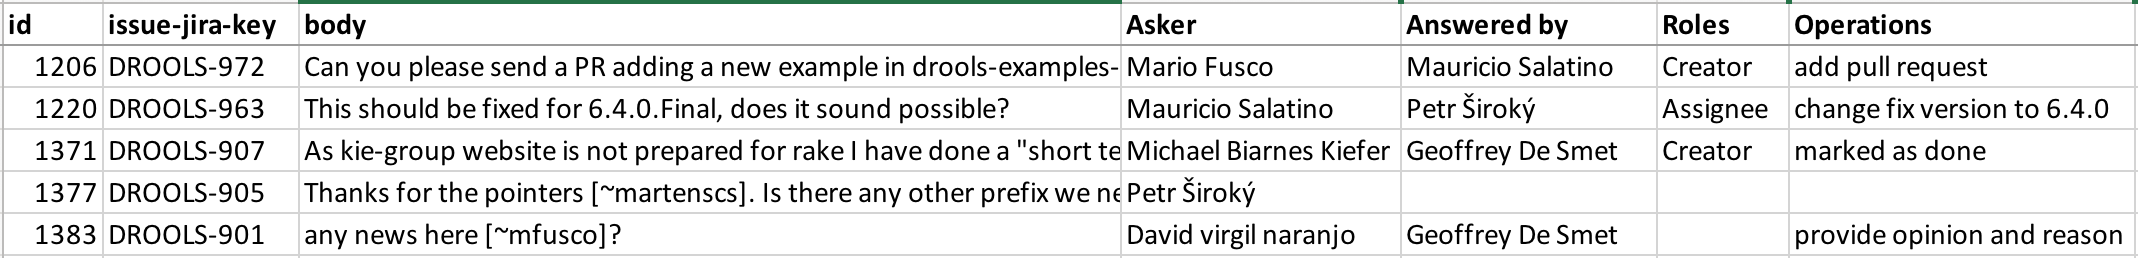
\includegraphics[width=\textwidth]{img/drools.png}
%   \caption{Select Questions with Identified Answer from DROOLS}
%   \label{fig:drools}
% \end{figure*}

\begin{table*}[!t]
  \centering
  \small
  \caption{Select Questions with Identified Answers from DROOLS}
  \tabcolsep=0.11cm
  \scalebox{0.82}{
    \begin{tabular}{ |l|l|l|l|l|l|l|  }
      \hline
      id & issue-jira-key & body & asker & answered by & role & operations \\
      \hline
      1206 & DROOLS-972 & Can you please send a PR adding a new example in \ldots & Mario Fusco & Mauricio Salatino & Creator & add pull request \\
      1220 & DROOLS-963 & This should be fixed for 6.4.0.Final, does it sound possible? & Mauricio Salatino & Petr Široký & Assignee & change fix version to 6.4.0 \\
      1371 & DROOLS-907 & As kie-group website is not prepared for rake I have \ldots & Michael Biarnes Kiefer & Geoffrey De Smet & Creator & marked as done \\
      1377 & DROOLS-905 & Thanks for the pointers [~martenscs]. Is there any   \ldots & Petr Široký & & & \\
      1383 & DROOLS-901 & any news here [\textasciitilde mfusco]? & David virgil naranjo & Geoffrey De Smet &  & provide opinion and reason \\
      1627 & DROOLS-823 & Hi Geoffrey, When an error is found, what would \ldots & Michael Biarnes Kiefer &  &  & \\  
      \hline
  \end{tabular}
  }
  \label{tab:drools}
\end{table*}


% =============================================================
% == Graphs ===================================================
% =============================================================
\section{Examining Requirements Socio-Technical Graphs}
In order to successfully create patches in a requirements traceability environment, we must first understand the characteristics of the environment. To do this, we construct graphs of the environment following the Codebook paradigm. We then examine the types of human-human and human-artifact relationships that connect a traceability question to an identified answer; encoding these relationships can build a patch that a requirements traceability forager can explore to understand their prey\textemdash their need to understand their traceability question\textemdash better.

\subsection{The Information Environment}
% - Why Jira?
The literature suggests that issue trackers are essential for open-source projects to manage requirements~\cite{ICSE5,ICSE25,ICSE33,ICSE40,ICSE60}. Although the requirements of an open-source project can originate from emails, how-to guides, and other socially lightweight sources~\cite{ICSE62}, the to-be-implemented requirements ``eventually end up as feature requests in an issue-tracking system''~\cite{ICSE33}. We therefore turn to the issue-tracking system Jira to understand the life of requirements.

% - Why 6 projects within Jira?
From Jira, we select four open-source projects from the Apache software foundation~\cite{ICSE7} or the JBoss family~\cite{ICSE38}.
The four projects tackle problems in different domains with implementations written in different programming languages, as seen in Table \ref{tab:jiraProjects}.

% - within projects, requirements manifest themselves as questions
Within the chosen projects, we focus on questions and answers. As discussed, questions represent a traceability forager's information need. By finding the exact person who answered a forager's question, we can gain insight into the information environment. For each project, two researchers identified comments that were questions and identified the respective answer comments, building their answer sets individually. Some examples of the answer sets generated can be seen in Table \ref{tab:drools}. The researchers reached a substantial degree of agreement (average Cohen's kappa=0.67) on requirements traceability questions over the 4 projects. Discrepancies were resolved in a joint meeting between the researchers. 

% - why do we considered these projects heterogeneously? 
% - what are our node types? issues, comments, and people.
In Jira, issues (typically tasks or feature requests) are our requirements. Comments are provided to the issue, and may contain questions or answers. Users create issues, are assigned to issues, submit comments, and reference other users within their comments. Contemporary approaches to requirements traceability are either artifact-based (e.g., trace retrieval) and would consider only the comments and issues~\cite{ICSE15}, or are driven by social roles (e.g., contribution structures in the requirements specification production) and would consider the relationships of the people~\cite{ICSE29}. As we constructed our answer set, however, we realized the impact of the people-artifact relationships on the ability to track a requirement's life. Therefore, we consider Jira's issues, comments, \textit{and} people in our information environment.

% For example, Petr’s question mentioned in Section 3.3 was very specific in terms of both the to-be-found artifact (jsr94 jar) and the people that he felt would be most helpful (Mario Fusco or Mark Proctor) [64]. Yet, the question was unanswered.
% Checking the contribution structures [30] of this DROOLS requirement [64] leads to the social network with only one node, i.e., Petr who reported/created and was assigned to work on the requirement. By expanding the contribution structures to also include artifacts in the Codebook fashion [11], the number of nodes increases, e.g., Petr’s comment containing the traceability question is added as an artifact node. Even in this socio-technical graph, the number of people nodes is rather small, with Petr, Mario, and Mark being involved. The inclusion of Mario and Mark is based only on the “mention” relationship of Petr and his comment. Our manual inspection of these three people in DROOLS suggests that they have relatively weaker connections among themselves, which in turn indicates that they may belong to different community-clusters.

\subsection{Constructing Requirements Socio-Technical Graphs}
The next step to creating patches in this network is to build a requirements socio-technical graph (RSTG) so that we can inspect the topology of the network using graph theory concepts. Issues, comments, and people serve as the nodes in our network. What, then, serve as the edges between our nodes?

\begin{figure}
	\centering
	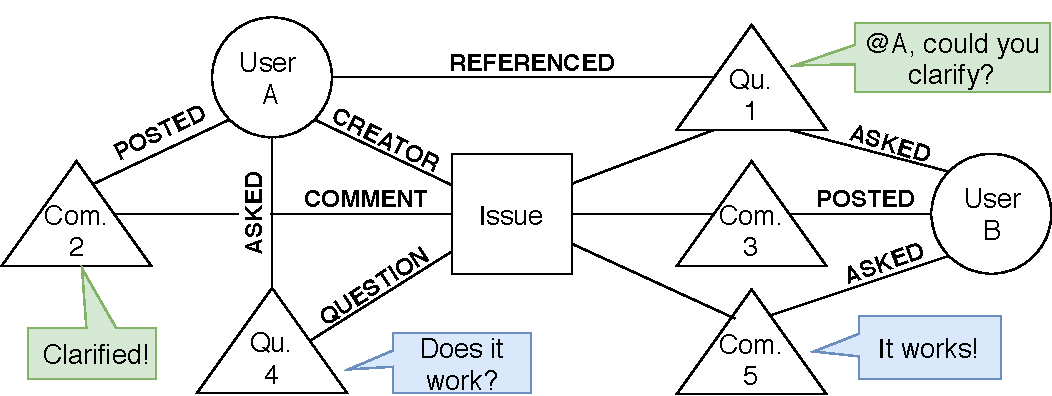
\includegraphics[width=\linewidth]{img/rstg.pdf}
	\caption{Requirements Socio-Technical Graph}
	\label{fig:rstg}
\end{figure}

By manually inspecting the paths between questions and their eventual answers, we are able to define the edges in our network topology. Consider the following example: Figure \ref{fig:rstg} is a subgraph from the IMMUNANT project, showing two questions and their answers. User 2881 created Issue 73650. User 6655, the forager, commented on the issue (Comment 149789), asking User 2881 for clarification by referencing them in the comment. User 2881 commented on the issue (Comment 149790), providing the clarification. In another foraging interaction, User 2881, now the forager, commented on the issue (Comment 149792), asking ``This is now available in [incremental build|http://immutant.org/builds/2x/] 591 and newer. Can you give that a try and confirm it works for you?'' User 6655 responded (Comment 149793) ``I've finally found the time to test this and can confirm it works! Thanks!''. 

These two foraging interactions demonstrate most of the observed relationships between nodes in the datasets. These relationships are treated as the edges within our graph:
\begin{itemize}
  \item \textit{Creator:} Users create issues
  \item \textit{Commented, Asked: }Users post comments and questions
  \item \textit{Comment, Question:} Comments and questions are posted to Issues
  \item \textit{Referenced:} Comments can reference other users
  \item \textit{Assignee:} (Not pictured) Users can also be designated assignees on issues 
\end{itemize}
While some relationships could be considered as unidirectional, e.g., a user posting a comment, the comment also serves as a bridge connecting the issue to the user, who is knowledgeable on the issue. We therefore elected to encode the network as an undirected graph.

By traversing the issues, comments, and users of each Jira project, and connecting each with these relationships, RSTGs like Figure \ref{fig:rstg} are constructed. An RSTG was constructed for each question, representing the state of the network at the time of the question. That way, only relationships that had existed prior to the asking of the question could be considered.

While each issue has its creator and assignee explicitly defined by Jira, and each comment has its author and issue, some additional processing was required to identify questions and references. Questions were identified by natural language recognition. In practice, a reference can either be the user's username (e.g., [\textasciitilde ge0ffrey]) or by first name (e.g., ``Geoffrey,'' or ``Geoffrey:''). With regular expressions, usernames were identified in the body of a comment and connected the comment to the user. However, first-name references had to be manually recognized and connected to their usernames. 

\subsection{Properties of Requirements Socio-Technical Graphs in Information Foraging}
We now tie our RSTGs to information foraging theory. When a forager asks a question, like the ones in Figure \ref{fig:rstg}, where do they find their answer? What path might the traceability forager typically follow to the user who will provide the answer, gathering information on their prey along the way?

\begin{figure}
	\centering
	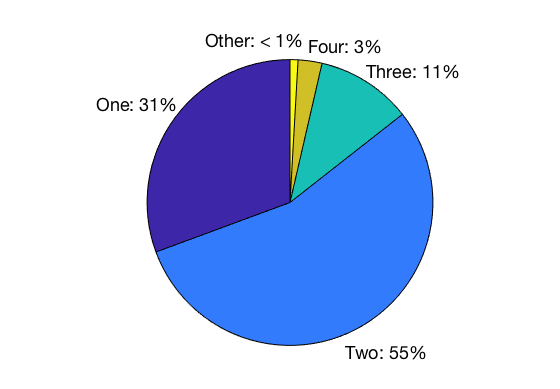
\includegraphics[width=\linewidth]{img/pie.png}
	\caption{Degrees of Separation between Question and Answer in Projects}
	\label{fig:pie}
\end{figure}

By analyzing the paths connecting question nodes and answer nodes, we identified recurring patterns connecting traceability questions with answers. The patterns are organized by degrees of socio-technical separation, which we define as the minimum number of edges to be traversed between two nodes. Figure \ref{fig:pie} displays the frequency of degrees separating questions and answers for our 111 questions. 

\subsubsection{One or Two Degrees of Separation}
Figure \ref{fig:pie} shows that more than three-quarters of answers are within two degrees of the question. These represent simple foraging tasks. By the time a forager posts a question, they may be relatively familiar with an issue. The very fact that they chose a specific issue to comment on demonstrates that they expect their answer to be near the issue. A well-informed forager will often reference the exact user they expect to know the answer. These kinds of relationships fall within this category.

\begin{figure}[ht]
	\centering
	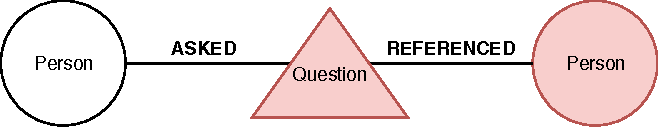
\includegraphics[width=0.9\linewidth]{img/1deg.pdf}
	\caption{Referenced (1 Degree)}
	\label{fig:1deg}
\end{figure}

Within one degree of the question, two types of answers were observed. The first is when the forager answers their own query. Because the forager, in the RSTG, is directly connected to their comment, this is one degree of separation. The second is when a user is referenced within a comment. As shown in Figure \ref{fig:1deg}, when a user is referenced in a comment, they are directly connected to the comment. Comment 70842, from the DROOLS project, is a good example of this: "What should the URL look like in your opinion [\textasciitilde tirelli]?" asks User 4079. User tirelli answers. A vast majority of the 31\% of answers one degree away from the question came from direct references.

\begin{figure}[ht]
	\centering
	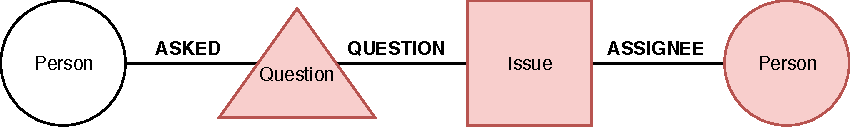
\includegraphics[width=0.9\linewidth]{img/2deg.pdf}
	\caption{Creator or Assignee (2 Degrees)}
	\label{fig:2deg}
\end{figure}

Within two degrees of separation, we observed two more types of answers: when a forager asks a question on an issue, either the issue creator or issue assignee responds. Figure \ref{fig:2deg} shows this interaction. When a forager posts a question to an issue without a reference, the creator, with their knowledge of what the issue is, or the assignee, with knowledge of what is being done to solve the issue, can answer. In Comment 353748, from the JBTM project, User 133 posts to an issue: ``Status update please?'' User 3619, assignee, provides an answer.

\subsubsection{Collaborators and Contributors\textemdash Three or Four Degrees of Separation}
More challenging foraging occurs when the user with the answer is three or more degrees of separation away from the question. With each degree, the number of information artifacts and other users a forager must traverse increases exponentially. Identifying patterns and presenting useful patches to the forager in this class of foraging presents far greater potential. We present a few of the most frequent types of interactions that occur within this radius. 

\begin{figure}[ht]
	\centering
	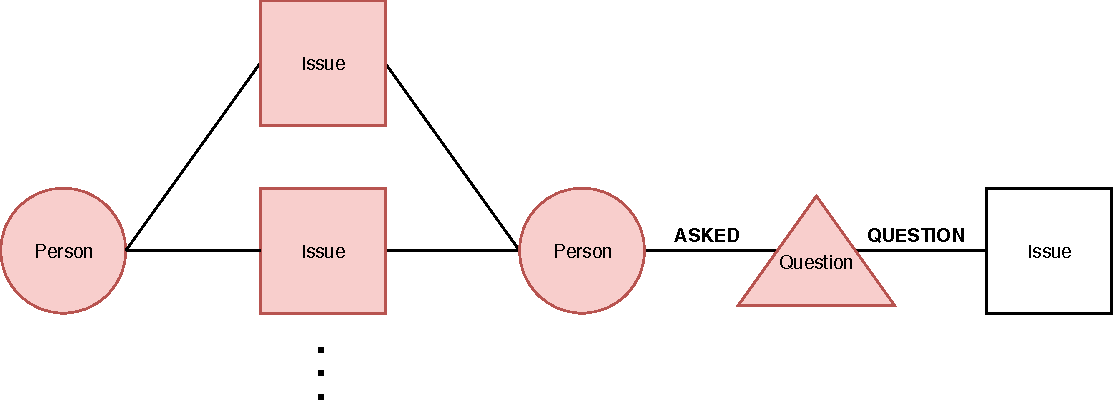
\includegraphics[width=\linewidth]{img/3degCollab.pdf}
	\caption{Frequent Collaborator of Asker or Referenced User (3 Degrees)}
	\label{fig:3degCollab}
\end{figure}

Most answers in our projects within three degrees of separation were of the type shown in Figure \ref{fig:3degCollab}: Comment--Person--Issue--Person. The question connects to a person\textemdash either the traceability forager or a referenced user\textemdash and the answer comes from a \textit{Frequent Collaborator}. While neither the forager themselves nor a referenced user has an answer, someone they collaborate with does. The Collaborator is connected with the user or the referenced by one or more comments (where the Collaborator is directly referenced). We notice that Collaborators are often highly-central users in a project, whose Frequent Collaborator status arises from their frequent contributions to projects. In other words, they are Frequent Collaborators because they are frequent users in general.

\begin{figure}[ht]
	\centering
	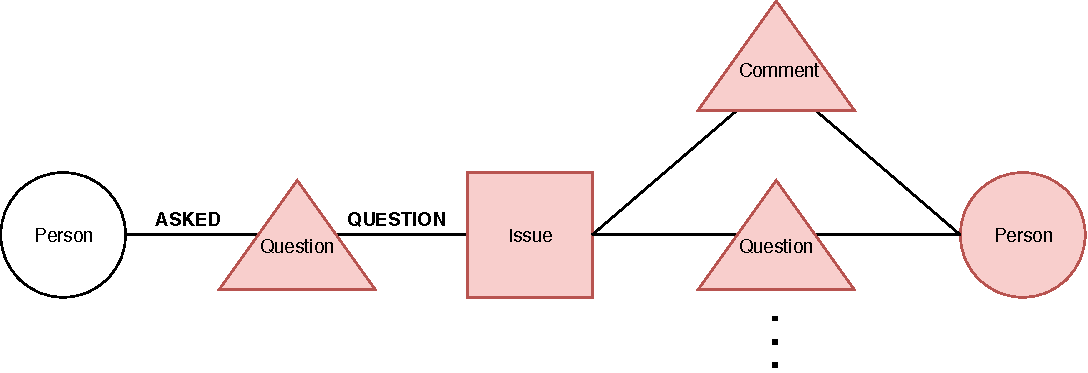
\includegraphics[width=\linewidth]{img/3degContrib.pdf}
	\caption{Frequent Contributor to Issue (3 Degrees)}
	\label{fig:3degContrib}
\end{figure}

The second type of answer within three degrees of separation is that shown in Figure \ref{fig:3degContrib}: Comment--Issue--Comment--Person. We call this type of answer a \textit{Frequent Contributor}. This user does not directly know the forager, nor are they creator or assignee of the issue. However, the Contributor has commented and asked on a given issue one or more times. Again, Frequent Contributors tend to be highly-active, and therefore highly-central users. Figure \ref{fig:pie} shows that Frequent Collaborators and Frequent Contributors represent 11\% of answers in our dataset.

\begin{figure}[ht]
	\centering
	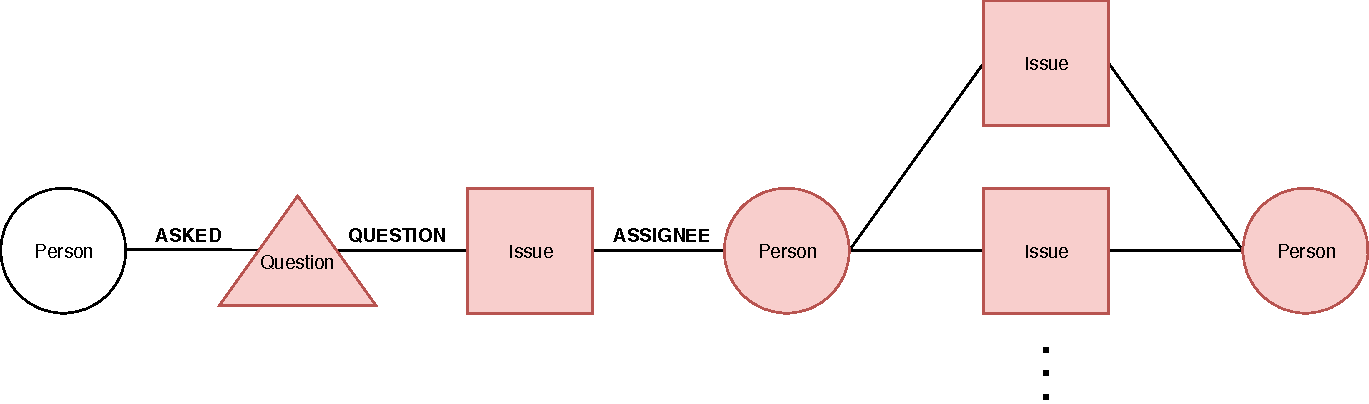
\includegraphics[width=\linewidth]{img/4degCollab.pdf}
	\caption{Frequent Collaborator of Creator or Assignee (4 Degrees)}
	\label{fig:4degContrib}
\end{figure}

Within four degrees, we see another variant of The Collaborator: a \textit{Frequent Collaborator of the Creator or Assignee} (Figure \ref{fig:4degContrib}). This type of relationship is signified by the pattern Comment--Issue--Person--Issue--Person. The creator or assignee of the issue has collaborated with the answerer on other issues before, either as creator or assignee on those issues. While the creator or assignee of the primary issue being considered may not have the answer, someone they often work with may. Figure \ref{fig:pie} shows that these kinds of interactions represent 3\% of our dataset.

We hypothesize that, within three or four degrees of separation, several other types of collaborators could be observed. Frequent Collaborators of the Asker could manifest by Comment--Person--Comment--Person, rather than Comment--Person--Issue--Person as we observed. Within four degrees, we observed Frequent Collaborators of Creators or Assignees; a Frequent Collaborator of the Asker could also show up within four degrees (Comment--Person--Issue--Comment--Person, or Comment--Person--Comment--Issue--Person). 


\subsubsection{Five or More Degrees of Separation}
In our sample set of 111 questions, there were no instances of five or more degrees of separation. Within this class, though, we hypothesize that more interesting variations of Frequent Collaborators and Frequent Contributors would arise; if one user does not know the answer, someone they know will. However, not having observed this class, we do not anticipate that it will be a commonplace sight.

\subsubsection{Disconnected Users}
\begin{figure}[ht]
	\centering
	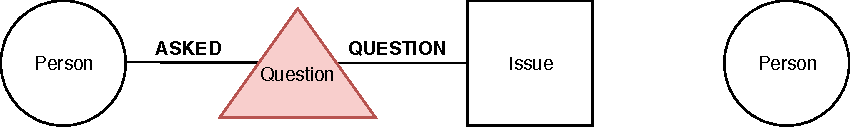
\includegraphics[width=0.9\linewidth]{img/disconnected.pdf}
	\caption{Answer disconnected from network}
	\label{fig:disconnected}
\end{figure}

The final pattern observed was one instance of an answer unconnected from the graph of the project (Figure \ref{fig:disconnected}). At the time the question was asked, the user who will eventually answer the forager's traceability question was not yet connected to the project by the relationships we chose to express as edges. When that user finally did connect to the the network, they were four degrees of separation away (Comment--Person--Comment--Issue--Person), appearing as the assignee to an issue where the asker had commented. With a larger dataset, these not-yet-connected relationships would be interesting to assess. More edge and node types could enable a connection between that user and the question.

\begin{table}[!ht]
	\caption{Number of Nodes Within N Degrees of Question}
	\centering
		\begin{tabular}{ |c||c|c|c|c|c|  }
		\hline
		& Min & Q1 & Med & Q3 & Max \\
		\hline
		1 Degree & 4.00 & 42.00 & 227.00 & 488.00 & 2461.00 \\
		2 Degrees & 5.00 & 278.00 & 575.50 & 1317.00 & 4166.00 \\
		3 Degrees & 5.00 & 567.00 & 1939.50 & 3177.00 & 7594.00 \\
		4 Degrees & 5.00 & 729.00 & 2686.50 & 4163.00 & 7953.00 \\
		\hline
	\end{tabular}
	\label{tab:radiusStats}
\end{table}
It appears, from these classes, that a substantial amount of traceability foraging takes place in four-or-less degrees of separation. Seeking to apply information foraging to traceability, one could simply present all nodes within three-to-four degrees of the question as a patch where the forager might seek to understand their question. This would satisfy our requirement of encoding frequently-traversed foraging paths into a patch. However, as shown in Table \ref{tab:radiusStats}, these patches are extremely large. With some notion of relatedness, however, these patches could be made smaller without losing relevant information.

% =============================================================
% == Patches ==================================================
% =============================================================
\section{Creating Socio-Technical Patches for Information Foraging}
In order to create smaller patches which still contain the described relationships, we turn to the foraging concept of scent. Following the example of WUFIS and PFIS,
we define the foraging concept \textit{Information Scent} as the ``inferred relatedness of a cue to the prey, as measured by amount of activation from a spreading activation algorithm.'' In WUFIS and PFIS, relatedness between two nodes was determined by a function of textual similarity and encoded into the weights of the edge connecting those two nodes. The application of spreading activation introduced a notion of proximity; each node's activation is representative of its textual similarity and proximity to the starting point\textemdash the information need. Our challenge is taking the work of WUFIS and PFIS and defining these concepts in our socio-technical context. Once we have a measure of relatedness in traceability foraging, we can create patches.

\subsection{Spreading Activation over Requirements Socio-Technical Graphs}
If a forager posts a question on an issue, the user who will provide the answer will likely require knowledge on that issue. From this postulate, we define our notion of ``relatedness'' between two nodes: the degree of a user's relatedness to an artifact is proportional to their knowledge on the artifact. This serves as an analogue to PFIS's textual similarity. The user's knowledge on an artifact is encoded as the weight on the edge connecting them. Note that, to support our implementation of spreading activation, a lower weight represents a more powerful connection.
\begin{itemize}
  \item \textit{Comment to Issue, Question to Issue:} \textbf{weight = 1}. This is the only type of artifact-to-artifact edge we defined in our RSTGs. If a comment or question is posted to an issue, it is directly a part of the traceability history of that issue. Therefore, its connection to the issue should be extremely strong.
  \item \textit{Creator to Issue, Assignee to Issue:} \textbf{weight = 2}. As discussed, the creator and assignee have a high degree of knowledge on a given issue. In relationships connecting question to answer, the assignee or creator frequently answered questions if the forager did not directly reference a user first (Figure \ref{fig:pie}: 55\% of questions). However, an issue can develop without the supervision of the creator or assignee. Therefore, the connection of this relationship is lower than that of an issue to a comment.
  \item \textit{Comment to Referenced:}  \textbf{weight = 2}. The user who wrote the comment has determined that the referenced user should have strong knowledge on the comment. Figure \ref{fig:pie} shows that 31\% of questions were answered by a referenced user; this relationship is therefore prioritized with a strong connection.
  \item \textit{Comment to User:} \textbf{weight = 3}. While the connection of a comment to the issue is strong, the user is not guaranteed to have knowledge on the issue to the same degree as Creator or Assignee. Therefore, we set the user's connection to the issue lower than that of a creator or assignee.
  \item \textit{Question to User:} \textbf{weight = 4}. Questions, like comments, do not guarantee knowledge on the issue. If anything, a user asking a question is least-qualified of the users discussed to provide an answer. Therefore, we give this relationship the weakest connection.
\end{itemize}

With weight defining the relatedness between two given nodes, now a given node's relatedness to the forager's information need can be determined. The classes discussed in the previous section demonstrated that answers fell within four degrees of separation, and that answers were likely to come from Frequent Collaborators. These concepts can be encoded by adapting spreading activation.

\begin{algorithm}
	\textbf{Spreading Activation}
	\begin{algorithmic}[1]
		\renewcommand{\algorithmicrequire}{\textbf{Input:}}
 		\renewcommand{\algorithmicensure}{\textbf{Output:}}
		\REQUIRE Graph, Source Node 
		\ENSURE Graph with Activated Nodes
		\STATE $Decay \leftarrow 0.1$
		\STATE $source.activation\leftarrow 1$
			\FOR{$node$ in Breadth-First Traversal from $source$}
				\FOR{$preNode$ in Neighbors of $node$}
					\IF{$preNode$ has been traversed}
						\STATE $weight \leftarrow edge(preNode,node)$
						\STATE $newActivation \leftarrow preNode.activation * (1 - weight * decay)$
						\STATE $node \leftarrow Activate(node, newActivation)$
					\ENDIF
				\ENDFOR
			\ENDFOR
	\end{algorithmic}
	~\\
	\textbf{Co-Routine: Activate}
	\begin{algorithmic}[1]
		\renewcommand{\algorithmicrequire}{\textbf{Input:}}
 		\renewcommand{\algorithmicensure}{\textbf{Output:}}
		\REQUIRE Node, New Activation
		\ENSURE Activated Node
		\STATE $frequencyReward \leftarrow 0.01$
		\IF{$node$ has activation}
			\STATE $maxAct \leftarrow max(node.activation, newAct)$
			\STATE $minAct \leftarrow min(node.activation, newAct)$
			\STATE $node.activation \leftarrow maxAct + ((1-maxAct) * minAct * frequencyReward)$
		\ELSE
			\STATE $node.activation \leftarrow newActivation$
		\ENDIF
	\end{algorithmic}
\caption{Spreading Activation over an RSTG}
\label{alg:spread}
\end{algorithm}

As shown in Algorithm \ref{alg:spread}, our variant of spreading activation starts at the question-node. The question's activation is set to 1. Then, surrounding nodes are traversed (Algorithm \ref{alg:spread}, Line 3), and activation is spread from their predecessors (Algorithm \ref{alg:spread}, Lines 4-8). Spreading activation traditionally has each node firing to its successors; our predecessor variant exhibits greater decay while still producing useful networks. Our exact mechanism of spreading activation is shown in Algorithm \ref{alg:spread}, Line 7, and the Algorithm \ref{alg:spread} Co-Routine.

Line 7 shows how exactly weight is factored in. A lower weight implies a higher degree of relatedness. If activation is a measure of relatedness, lower weights should result in higher activations. Therefore, the lower the weight, the smaller the effect of the decay, and the higher the resulting activation.

\begin{figure}[ht]
	\centering
	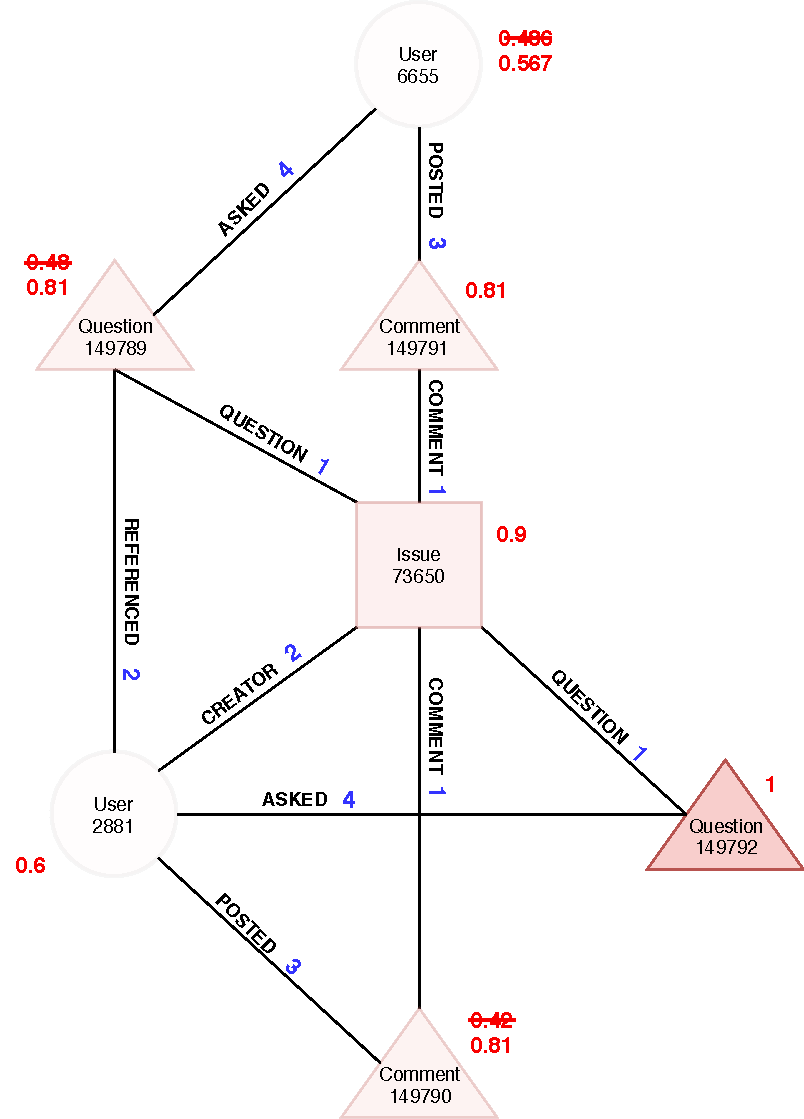
\includegraphics[width=0.85\linewidth]{img/RSTG-SA.pdf}
	\caption{Spreading Activation Applied to an RSTG (Without Frequency Bonus)}
	\label{fig:rstg-sa}
\end{figure}



The co-routine is divided into two branches by a conditional structure (Algorithm \ref{alg:spread}, Co-Routine, Line 2). If a node has no activation yet, the activation is simply spread to the new node. However, if a node already has activation, which activation is considered? Following the example of PFIS2~\cite{pfis2}, the higher activation value is spread. However, in order to incentivize frequency (in order to promote the Frequent Collaborator and Frequent Contributor patterns), if a node already has activation (i.e. the node has an existing relationship to the question), a percentage of that existing relationship is added to the new activation. Currently, this frequency reward is set to 1\% (Algorithm \ref{alg:spread}, Co-Routine, Line 1); otherwise, highly-central figures gained disproportionately high activations, and therefore activations did not suitably diminish throughout the graph. Another method for reinforcing frequent collaboration could be a subject for future work.

Figure \ref{fig:rstg-sa} provides an example of this variant of spreading activation being applied to the RSTG from Figure \ref{fig:rstg}. Each of the relationships is assigned its weight, and the activation of Question 149792 is set to 1. Then, User 2881 and Issue 73650 are visited and activation from the question is spread. Comment 149790 and Question 149789 had activation spread from both User 2881 and Issue 73650; the higher activation was retained. 

\subsection{Delineating Patches within Spreading Activation RSTGs}
With spreading activation encoding relatedness with the traceability forager's information need, patches can be created. Recall, from WUFIS and PFIS, that activation is a measure of information scent. By grouping together nodes with high activation, a patch with nodes related by the relationships described previously will be created. To do this, though, a threshold of ``high'' activation must be defined.

Earlier, creating patches by simply enclosing all nodes within four degrees of separation was proposed, because all answers in our dataset fell within four degrees. We now consider those answers' activations. Examining graphs of the classes discussed earlier, with spreading activation completed, reveals that a forager setting the cutoff at 0.72 would include 84\% of results. Setting the cutoff at 0.45 would include all results. Examining earlier classes revealed that many Frequent Contributors and their related information artifacts fall above 0.56; many Frequent Collaborators fall around 0.50.

\section{Results and Analysis}
\subsection{Quantitative Evidence}
The descriptive statistics in Table \ref{tab:resultsStats} suggest that delineating patches by activation creates smaller patches than by degrees of separation (Table \ref{tab:radiusStats}). Statistically comparing 4 Degrees and Activation $\geq$ 0.45, we conclude that the two sets are non-identical (t = 10.901, p-value $<$ 0.01). A similar test for Activation $\geq$ 0.45 and $\geq$ 0.72 reaches the same conclusion (t = 9.6481 p-value $\geq$ 0.01). In other words, each cutoff has significantly smaller patches than the previous. 

\begin{table}[ht]
	\caption{Patch Size With Cutoff}
	\centering
	\begin{tabular}{ |c||c|c|c|c|c||c|  }
		\hline
		& Min & Q1 & Med & Q3 & Max & Answer \\
		\hline
			4 Degrees & 5 & 729 & 2686 & 4163 & 7953 & 100\% \\
			A $\geq$ 0.45 & 5 & 273 & 649 & 1860 & 4834 & 100\% \\
			A $\geq$ 0.72 & 2 & 4 & 6 & 10 & 24 & 84\% \\
		\hline
	\end{tabular}
	\label{tab:resultsStats}
\end{table}

While patch sizes at cutoff Activation $\geq$ 0.45 are still too big for timely foraging, patch sizes at $\geq$ 0.72 are substantially more reasonable. That being said, $\geq$ 0.72 patches frequently do not include the answer node for three or four degree of separation relationships. However, within these patches, we believe that foragers would still find information relevant to their information need.

\subsection{A Practical Example}
Figure \ref{fig:rstg-sa} serves as a practical example of both the mechanism of the algorithm and a tradeoff to consider. Figure \ref{fig:rstg-sa} is a network with a cutoff set to $\geq$ 0.56\textemdash a cutoff chosen for its inclusion of many Frequent Contributors. Indeed, it was a Frequent Contributor that answered User 2881's question; User 6655 had commented twice on Issue 73650 already. While the question (``Does it work?'') was a pointed request, asking for a specific piece of information, the patch generated by the request yields not only the user who will answer the request, but also related traceability information. 

Figure \ref{fig:rstg-sa} also demonstrates a limitation of the algorithm in its current state. Other implementations of spreading activation begin from one or more nodes; we could have started the activation from the question \textit{and} the asking user. We chose to include only the question node, as to avoid superfluous information from the asking user's connections. In this case, though, had we included User 2881 as an initial node for activation, the algorithm would have assigned higher activations to the direct collaboration between User 6655 and User 2881 (User 2881--Question 149789--User 6655). This collaboration was key to the traceability history of Issue 73650.

%\subsection{Limitations}


% =============================================================
% == Implications =============================================
% =============================================================
\section{Implications}

%We discuss in this section the implications of our work as well as the limitations of our study.
Piorkowski and his colleagues~\cite{navValueCost} codified the fundamental challenges faced by software developers when foraging in the information environment. We believe that our socio-technical approach can help directly address the challenge of ``prey in pieces'' where the foraging paths were too long and disconnected by different topologies. By explicitly integrating humans in the underlying topology, information foragers can exploit a richer set of relationships.

Codebook~\cite{codebook10} confirmed that the small-world phenomenon~\cite{Chakrabarti-CSUR06} was readily observed in the socio-technical networks built from the software repositories, e.g., any pair of stakeholders would be connected in six-or-less hops. Our findings suggested that the requirements-centric socio-technical graphs are even smaller with relevant nodes surrounded in four-or-less degrees of separation from the traceability forager's question. Meanwhile, our results revealed several common relationships and their compositions. In light of the recent work on collecting practitioners' natural-language requirements queries (e.g.,~\cite{Pruski-REJ15, Lohar-REFSQ16, Malviya-RE17}), the patterns uncovered by our study could be used to better classify and answer project stakeholders' traceability needs.

Automated requirements traceability tools have been built predominantly by leveraging text retrieval methods~\cite{ICSE15}. These tools neglect an important factor\textemdash familiarity\textemdash which plays a crucial role in tracking the life of a requirement. Our work further points out that familiarity is multi-faceted: it could be the person familiar with the issue, the project, or the asker that is knowledgeable about the traceability information. Our results here are to be contrasted with the empirical work carried out by Dekhtyar \emph{et al.}~\cite{Dekhtyar-RE11} showing that experience (e.g., years worked in software industry) had little impact on human analysts' tracing performance. While a developer's overall background may be broad, we feel that the specific knowledge about the subject software system and the latent relationships established with project stakeholders do play a role in requirements tracing. Automated ways of inferring a developer's knowledge degree (e.g.,~\cite{Fritz-TOSEM14}) would be valuable when incorporated in traceability tools.

Requirements traceability serves as a critical case~\cite{yin03} for our investigation into developers' information foraging in a socio-technical environment. This is because, without the traceability information, many software engineering activities cannot be undertaken, such as verification that a design satisfies the requirements, validation that requirements have been implemented, change impact analysis, system level test coverage analysis, and regression test selection~\cite{Hayes-TSE06}. However, requirements traceability is by no means the only case. In fact, due to information foraging theory's parsimony, its constructs (e.g., patch and scent) have been adapted to support a variety of tasks including debugging, refactoring, and software reuse~\cite{Fleming-TOSEM13, Ragavan-CHI16, Ragavan-CHI17}. The socio-technical patch created by our spreading activation algorithm, therefore, could help developers answer their needs beyond requirements traceability.


%\begin{itemize}
%	\item \textit{Foraging and navigations, fundamentally developers predictions of value and cost}. Prey in pieces, path too long, no path across different topologies
%\end{itemize}


% =============================================================
% == Conclusion ===============================================
% =============================================================
\section{Conclusion and Future Work}
By considering common relationships connecting a requirements traceability question to its answer, and encoding these relationships into a spreading activation algorithm, we were able to delineate patches for use in understanding context surrounding requirements traceability questions in a socio-technical environment. In this process, we found that traceability questions were answered by users within four degrees of socio-technical separation; these users were typically Frequent Collaborators of the traceability forager or of the creator/assignee of the issue, or Frequent Contributors to the issue. Encoding these relationships as parameters to a spreading activation algorithm resulted in patches of nodes that a traceability forager could traverse, searching for their answer. While simply creating patches including all nodes within four degrees of socio-technical separation would include all answers, the addition of spreading activation created significantly smaller patches.

This method can further be extended within the requirements traceability realm. With only three node types\textemdash issues, comments, and people\textemdash we were able to generate these patches. With a higher diversity of information, such as code artifacts and commits, or semantic similarity, more nuanced relationships could be determined, and our process could be improved.

Future work could be conducted on the implementation of the algorithm itself, too. Our decay, frequency reward, and patch cutoff parameters were set through observation and trial and error. More sophisticated statistical analyses, like machine learning algorithms, could help better set these parameters. Our method only suggested the first patch for foraging; in reality, a forager will go through several patches in search of their prey. To accommodate this pattern, this work could be extended to multiple-patch creation. 

Most importantly, this method could easily be extended to other socio-technical tasks. In socio-technical tasks, such as comments and responses, we anticipate that a graphical analysis would reveal key relationships that could be considered when constructing patches. Applying spreading activation allows knowledge, proximity, and frequency, among other factors, to be encoded into the patch creation.

% \section*{Acknowledgment}
% To the researchers who created our answer sets and databases.


\bibliographystyle{IEEEtran}
\bibliography{VLHCC18-bib} 

\end{document}'